% \documentclass[review]{siamonline1116}
\documentclass[twocolumn,10pt]{asme2ej}
% \usepackage{geometry} % see geometry.pdf on how to lay out the page. There's lots.
% \usepackage{hyperref}
\usepackage{graphicx}
\usepackage{gensymb}
% \usepackage[affil-it]{authblk}
% \usepackage[toc,page]{appendix}
% \usepackage{pifont}
\usepackage{amsmath}
% \usepackage{amsthm}
\usepackage{amsfonts}
\usepackage{hyperref}
\usepackage{cleveref}

% \usepackage{float}

\newtheorem{theorem}{Theorem}
\newtheorem{corollary}{Corollary}
\newtheorem{lemma}{Lemma}

\newcommand\numberthis{\addtocounter{equation}{1}\tag{\theequation}}

\renewcommand{\vec}[1]{\mathbf{#1}}

% \usepackage{draftwatermark}



% \SetWatermarkText{DRAFT}
% \SetWatermarkScale{6}
% \SetWatermarkLightness{0.95}

% \geometry{letter} % or letter or a5paper or ... etc
% \geometry{landscape} % rotated page geometry

% See the ``Article customise'' template for come common customisations

\title{Untwisting the Boerdijk-Coxeter Helix}
\author{Robert L. Read
  \affiliation{
    Founder, Public Invention \\
    Austin, TX, 78704 \\
    Email: \href{mailto:read.robert@gmail.com}{read.robert@gmail.com} 
    }
}



\date{\today}

%%% BEGIN DOCUMENT
\begin{document}

\maketitle

%% \tableofcontents


%% TODO: Add something about Tetrobots into abstract.
\begin{abstract}
  The Boerdijk-Coxeter helix (BC helix, or tetrahelix) is a
  face-to-face stack of regular tetrahedra forming a helical column.  Considering the edges of
  these tetrahedra as structural members, the resulting structure is attractive and
  inherently rigid, and therefore interesting to architects,
  mechanical engineers, and roboticists.  A formula is developed that matches the
  visually apparent helices forming the outer rails of the BC helix.
  This formula is generalized to a formula convenient to designers.
  Formulae for 
  computing the
  parameters that give proven edge-length minimax-optimal tetrahelices
  are given, defining a continuum of optimum tetrahelices of varying curvature.
  The endpoints of this continuum are the BC helix and
  a structure of zero curvature, the \emph{equitetrabeam}.
  Only one out of three members in the system change their length to reach
  any point in the continuum.
  Numerically finding the rail angle from the equation for
  pitch allows optimal tetrahelices of any pitch to be designed. 
  An interactive tool for such design and experimentation is provided: \url{https://pubinv.github.io/tetrahelix/}.
  A formula for the inradius of optimal tetrahelices is given.
  The continuum allows a regular Tetrobot supporting a length change of less than $16\%$ in the
  BC configuration to untwist into a hexapodal or $n$-podal robot
  to use standard gaits.
\end{abstract}


%% \begin{keywords}
%%   Boerdijk-Coxeter helix, tetrahelix, robotics, tetrobot, unconventional robots,
%%   structural engineering, mechanical engineering, tensegrity, variable-geometry truss
%% \end{keywords}
%% \begin{AMS}
%%   51M15
%% \end{AMS}




\section{Introduction}

The Boerdijk-Coxeter helix\cite{coxeter1985simplicial} (BC helix) (see \cref{fig:closeup,fig:closeuporthog}), is
a face-to-face stack of tetrahedra that winds about a straight axis.
Architects, structural engineers, and roboticists are inspired
by and follow such regular mathematical models.
However, since they can also build structures and
machines of differing or even dynamically changing length, it is
useful to develop the mathematics of structures formed from tetrahedra
where we relax regularity.


The vertices of the tetrahedra lie upon
three helices about the central axis.
The 
Tetrobot\cite{readglussbot,TetrobotBook} uses the regularity of
this geometry to make a tentacle-like robot that can crawl like a slug
or mollusk.  These modular robotic systems use mechanical actuators which can
change their length, connected by special joints,
such as the 3D printable Song-Kwon-Kim\cite{song2003spherical} joint or the CMS joint\cite{HamlinSandersonCMS}
used in the original Tetrobot.
This allows many members to meet in a single point.
Such machines can
follow purely regular mathematical models such as the Boerdijk-Coxeter
helix or the Octet Truss\cite{richard1961synergetic}.

Buckminster Fuller called the BC helix a \emph{tetrahelix}\cite{fuller1982synergetics},
a term now commonly used. In this paper, we reserve \emph{BC helix} to mean the purely regular structure and use \emph{tetrahelix} to refer
to any structure isomorphic to the BC helix.

\begin{figure}
  \centering
     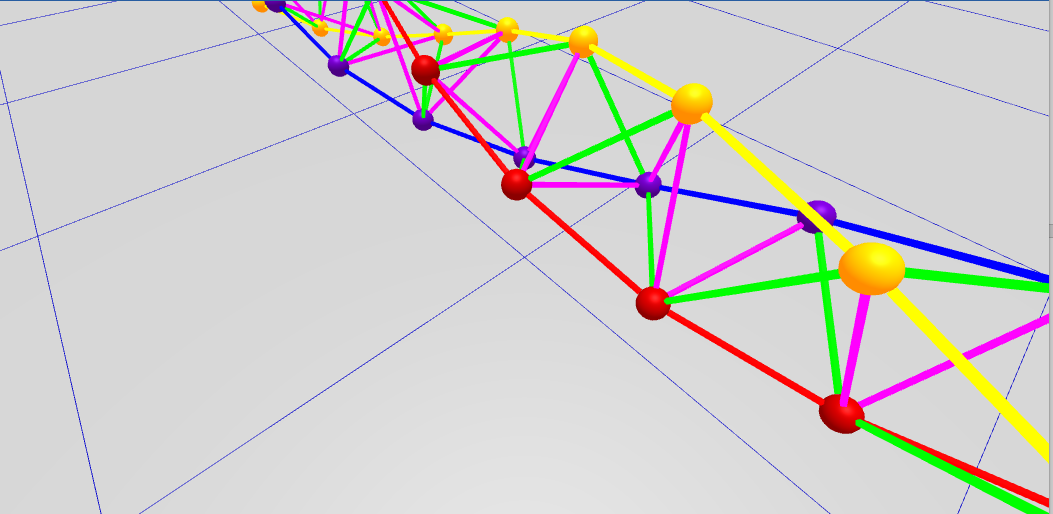
\includegraphics[width=0.45\textwidth]{figures/BCHelixCloseUp.png}
     \caption{BC Helix Close-up (partly along axis)}
  \label{fig:closeup}     
\end{figure}
\begin{figure}
  \centering
     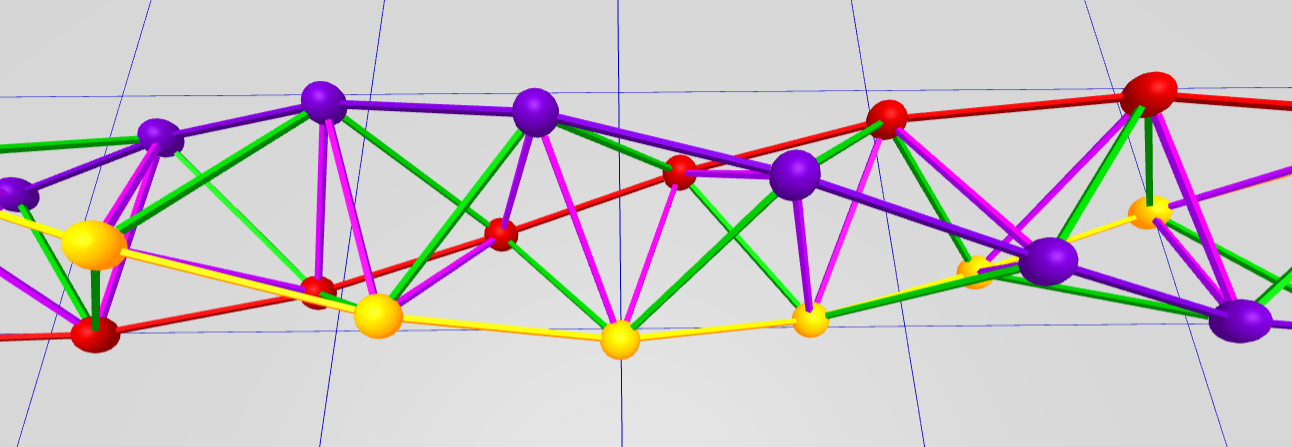
\includegraphics[width=0.45\textwidth]{figures/VerticalCloseUp.png}
     \caption{BC Helix Close-up (orthogonal)}
  \label{fig:closeuporthog}
\end{figure}

Imagining \cref{fig:closeup} or \cref{fig:closeuporthog} as a static mechanical structure,
we can observe that it is useful to the mechanical engineer
because the structure is a mechanically strong, inherently rigid,
omni-triangulated space frame.
Then we can imagine that each static edge is replaced with an
actuator that can dynamically become shorter or longer in response to electronic control,
and the vertices are joints that support sufficient angular displacement
for this to be possible. An example of such a machine is a Tetrobot,
shown in \cref{fig:tetrobot}.

A BC helix does not rest stably on a plane. It is convenient to
be able to ``untwist'' it and to form a tetrahelix space frame that has a
flat planar surface. By making length changes in a certain way, we can
untwist a tetrahelix to form a \emph{tetrabeam} which has planar faces
and has, for example, an equilateral triangular profile. This paper
develops the equations needed to untwist the tetrahelix. All math
developed here is available in JavaScript and demonstrated by an interactive
design website \url{https://pubinv.github.io/tetrahelix/}\cite{readtetrahelix},
from which \cref{fig:closeup,fig:closeuporthog} and later figures in this paper 
are taken.

\begin{figure}
  \centering
     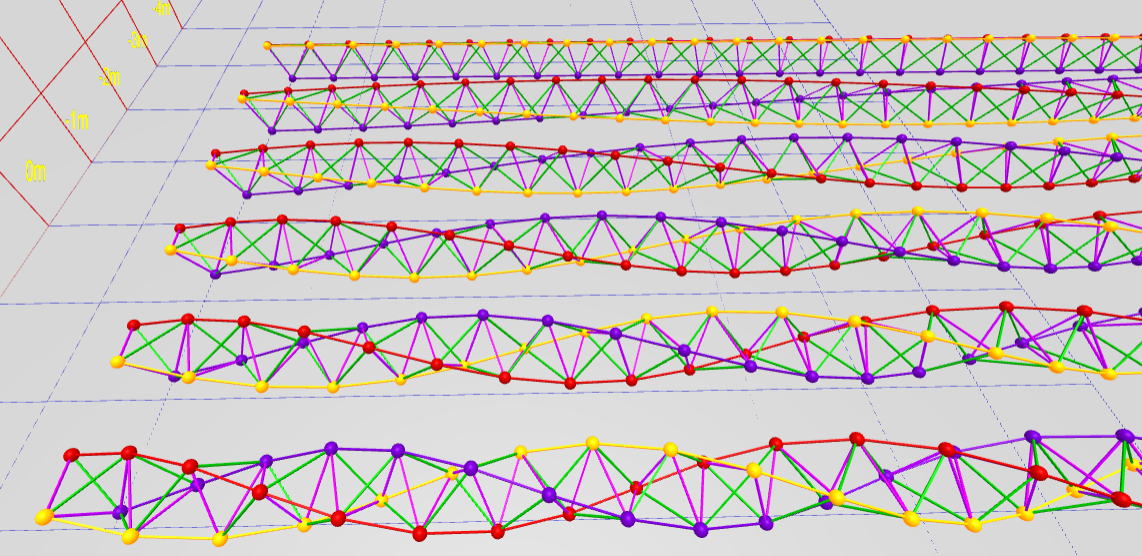
\includegraphics[width=0.45\textwidth]{figures/TetrahelixSeries2.png}
     \caption{A Continuum of Tetrahelices}
  \label{fig:series}
\end{figure}


\Cref{fig:series} displays a continuum of tetrahelices optimal in a certain sense,
which is the main result of this
paper. The closest helix is the BC helix, and the furthest
is the equitetrabeam, defined in \cref{sec:equitetrabeam} and \cref{fig:naming,fig:equitetrabeam}.

\section{A Designer's Formulation of the BC Helix}

We would like to design nearly regular tetrahelices with a formula that
gives the vertices in space. Eventually, we would like to design them
by choosing the lengths of a small set of members.
In a space frame, this is a static design choice; in a tetrobot, it is a
dynamic choice that can be used to twist the robot and/or exert linear or
angular force on the environment.

Ideally, we would have a simple formula for defining the vertices based on
any curvature or pitch we choose. It is a goal of
this paper to relate the Cartesian coordinate approach and the member-length approach to
generating a tetrahelix continuum.


H.S.M Coxeter constructs the BC helix\cite{coxeter1985simplicial} as a repeated rotation and translation of the tetrahedra by showing the
rotation is:
\begin{equation}
\theta_{bc} = \arccos(-2/3) 
\end{equation}
and the translation:
\begin{equation}
h_{bc} = 1/\sqrt{10}.
\end{equation}

Note that $\theta_{bc}$ is approximately $0.37 \cdot 2 \pi$ radians or  $131.81$ degrees.
The angle $\theta_{bc}$ is the rotation of \emph{each} tetrahedron, not the tetrahedra along a rail.  In \cref{fig:closeup},
each tetrahedron has either a yellow, blue, or red outer edge or rail.
That is, a blue-rail tetrahedron is rotated slightly more than a $1/3$ of a revolution to match the face of the yellow tetrahedron.

R.W. Gray's website\cite{graytetrahelix}, repeating a formula by Coxeter\cite{coxeter1985simplicial} in a more accessible form, gives the Cartesian coordinates $\begin{bmatrix}
           x \\
           y \\
           z
         \end{bmatrix}$
for a counter-clockwise BC Helix in a right-handed coordinate system:
\begin{equation}
  \label{graycoxeter}
\vec{V}(n) =
\left [
  \begin{tabular}{c}
   $ r_{bc} \cos{n \theta_{bc}} $\\
   $ r_{bc} \sin{n \theta_{bc}} $\\
   $ n h_{bc}  $
  \end{tabular}
  \right ],
\end{equation}
\text{where: \qquad}
  \begin{tabular}{l}
 $ r_{bc} = \frac{3\sqrt{3}}{10} \approx 0.5196 $,\\
 $ h_{bc} = 1/\sqrt{10} \approx 0.3162 $, and \\
 $ \theta_{bc} = \arccos(-2/3) $  \text{,}\\
  \end{tabular}      

and $n$ represents each integer numbered vertex in succession on the $z$-axis.

The apparent rotation of a vertex on an outer-edge, that is $\vec{V}(n)$ relative from $\vec{V}(n+3)$
for any integer $n$
in \cref{graycoxeter}, is $3 \theta_{bc} - 2\pi$.

This formula defines a helix, but it is not any of the apparent helices, or \emph{rail} helices, of the
BC helix, but rather one that winds much more rapidly through all
vertices. To a designer of tetrahelices, it is more natural to think of
the three helices which are visually apparent, that is, those three
which are closely approximated by the outer edges or rails of
the BC helix. We think of each of these three rails as being a different color: red, blue, or yellow.
This situation is illustrated in \cref{fig:helixcomparison}, wherein the black helix represents that
generated by \cref{graycoxeter},
and the colored helices are generated by \cref{eq:colored}, below. 



In order to develop the continuum of slightly irregular tetrahelices,
we need a formula that gives us the vertices of just
one rail helix, denoted by color $c$ and integer vertex number $n$:
\[
(\forall n \in \mathbb{Z}, \forall c \in \{0,1,2\} : \vec{H}_{BCcolored}(n,c) = \vec{V}(3n +c)) .
\]

Such a helix can be written:
\begin{equation}
  \label{eq:colored}
 \vec{H}_{BCcolored}(n,c) =
\left [
  \begin{tabular}{c}
   $ r_{bc}  \cos{((3 \theta_{bc} - 2 \pi)n + c  \theta_{bc})}  $\\
   $ r_{bc} \sin{((3 \theta_{bc} - 2 \pi)n + c  \theta_{bc})} $\\
   $ 3 h_{bc} (n + c/3)  $
  \end{tabular}
  \right ],
\end{equation}
\text{where:  \qquad}
  \begin{tabular}{l}
 $ r_{bc} = \frac{3\sqrt{3}}{10} $,\\
 $ h_{bc} = 1/\sqrt{10} $, and \\
 $ \theta_{bc} = \arccos(-2/3) $ \text{.}\\
  \end{tabular}      

In this formula, integral values of $n$ may be taken as a vertex number for one rail and used to compute
its Cartesian
coordinates. Allowing $n$ to take non-integer values defines a continuous
helix in space which is close to the segmented polyline of the outer
tetrahedra edges, and equals them at integer
values.

\begin{figure}
  \centering
     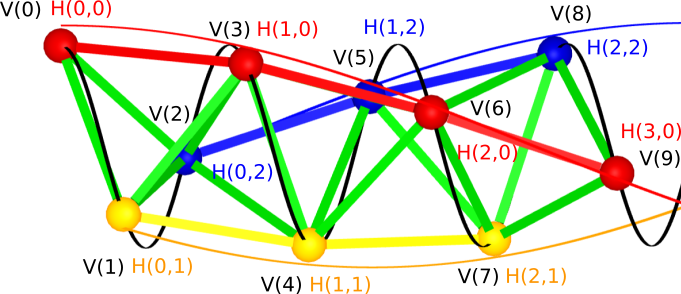
\includegraphics[width=0.45\textwidth]{figures/Unified.png}
     \caption{Rail helices (H) vs. Coxeter/Gray helix (V) }
  \label{fig:helixcomparison}  
\end{figure}

\Cref{fig:helixcomparison} illustrates this difference with a 7-tetrahedra BC helix, which is
in fact the same geometry as the robot illustrated in \cref{fig:tetrobot}.
Although the vertices coincide,
 \cref{graycoxeter} evaluated
at real values generates the black helix which runs through every vertex, and \cref{eq:colored} defines
the red, yellow, and blue helices. In this figure,
these rail helices have been rendered at a slightly higher radius than the vertices for clarity;
in actuality, the maximum distance between the continuous, curved helix and the
straight edges between vertices is much smaller than can be clearly rendered.

The quantity $ (3 \theta_{bc} - 2 \pi) \approx 35.43 \degree $  is the angular shift between
adjacent vertices on the same rail:
$ \vec{V}(3n + c)= \vec{H}_{BCcolored}(n,c)$ and
$ \vec{V}(3(n+1)+c)= \vec{H}_{BCcolored}(n+1,c)$.
This quantity appears so often that we call it the ``rail angle, $\rho$''. For the BC helix, $\rho_{bc} = (3 \theta_{bc} - 2 \pi)$.

\begin{figure}
     \centering
     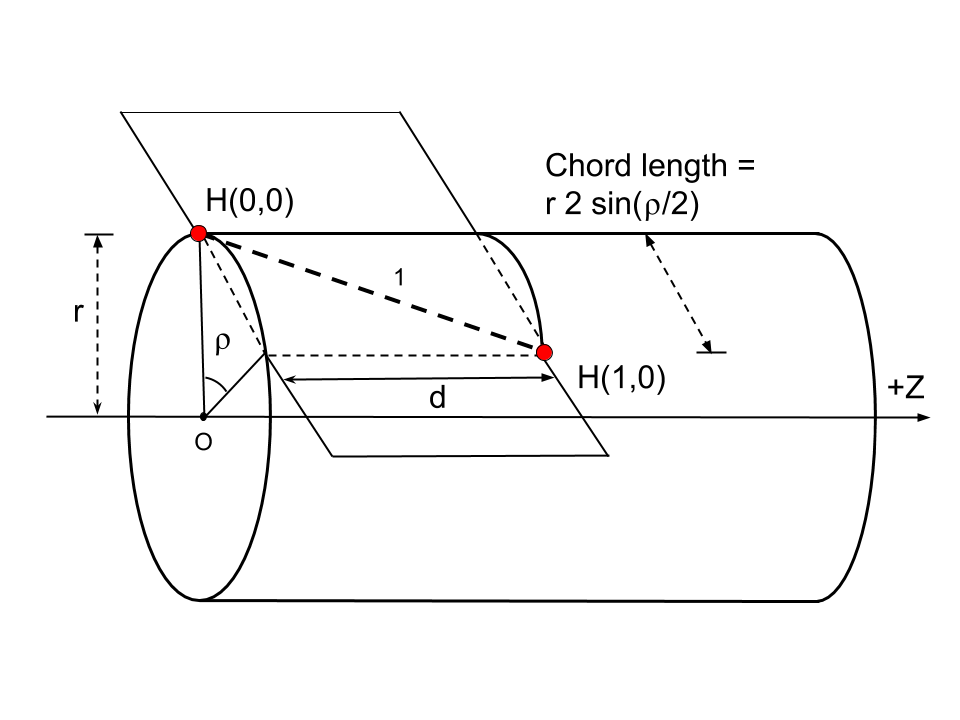
\includegraphics[width=0.45\textwidth]{figures/RailAngleGeometry.png}
     \caption{Rail Angle Geometry}
  \label{railanglefig}
\end{figure}

Note, in \cref{railanglefig}, the $z$-axis travel for one rail edge is denoted by $d$. In \cref{graycoxeter} and  \cref{eq:colored}, the variable
$h$ is used for one third of the distance, we name $d$. We will later justify that $d = 3h$.
In this paper, we assume the length of a rail
is always $1$ as a simplification, except in proofs concerning rail length.
We make the rail length a parameter in our JavaScript code in
\url{https://github.com/PubInv/tetrahelix/blob/master/js/tetrahelix_math.js} \cite{readtetrahelix}.

The $\vec{H}_{BCcolored}(n,c)$ formulation can be further clarified by rewriting directly in terms of the rail angle $\rho_{bc}$ rather than $\theta_{bc}$.
Intuitively, we seek an expression where $c/3$ is multiplied by a $1/3$ rotation plus the rail angle $\rho$.
We expand 
the expressions $\theta_{bc}$ and $\rho_{bc}$ in \cref{eq:colored} and seek to isolate the term $c 2\pi/3 $.


%% Thus:
%% \begin{align*}
%%  c \theta_{bc}  &=   \text{\{we aim for 3 in denominator, so we split...\}} \\
%%     (c/3)  (3 \theta_{bc})  &=   \text{\{we want $2\pi$ in numerator, so add canceling terms...\}} \\
%%  (c/ 3) ((3 \theta_{bc} - 2 \pi)  + 2 \pi) &= \text{\{definition of $\rho_{bc}$\ ...\}} \\  
%%   (c / 3) \rho_{bc}  + c 2 \pi /3 &=  \text{\{algebra...\}} \\  
%% c  ( \rho_{bc} +  2 \pi) /3 \text{ .} \\
%% \end{align*}


Thus, starting with the expression:
\begin{align*}
  c \theta_{bc} 
\end{align*}
we introduce 3 into the denominator...
\begin{align*}
  (c/3)  (3 \theta_{bc}) 
\end{align*}
we want $2\pi$ in numerator, so add canceling terms...
\begin{align*}
  (c/ 3) ((3 \theta_{bc} - 2 \pi)  + 2 \pi) 
\end{align*}
...and then use the definition of $\rho_{bc}$
\begin{align*}
  (c / 3) \rho_{bc}  + c 2 \pi /3 
\end{align*}
finally we obtain:
\begin{equation}
  c  ( \rho_{bc} +  2 \pi) /3  \text{.}
\end{equation}  

This allows us to redefine:

%% Actually, I am not sure if this is a clearer formulation...it might be, and need to put it in general!!!
\begin{equation}
\vec{H}_{BCcolored}(n,c) =
\left [
  \begin{tabular}{c}
    $ r  \cos{\rho_{bc} n + c (\rho_{bc} +  2 \pi) /3} $\\
   $ r  \sin{\rho_{bc} n + c (\rho_{bc} +  2 \pi) /3} $\\
   $ (n+c/3)  h_{bc} $
  \end{tabular}
  \right ],
\end{equation}
\text{where: \qquad}
  \begin{tabular}{l}
%%  $\kappa = n + c/3$ \\
    $\rho_{bc} = (3 \theta_{bc} - 2 \pi)$, and \\
    $ h_{bc} = 1/\sqrt{10} $. \\    
  \end{tabular}      


Recall that $c \in \{0,1,2\}$, but $n$ is continuous (rational or real-valued).
We can now assert that in \cref{fig:helixcomparison} the black helix winds at
$\frac{3 \theta_{bc}}{\rho_{bc}} \approx 11.16 $ times the rate of a rail helix.

From this formulation it is easy to see that moving one vertex on a rail
($\vec{H}_{BCcolored}(n,c)$ to $\vec{H}_{BCcolored}(n+1,c)$ for any $n$ and $c$)
moves us $\rho_{bc}$ radians around a circle. Since:
$ \frac{2 \pi}{\rho_{bc}} \approx 10.16 $
we can see that there are approximately $10.16$ red, blue or yellow tetrahedra on one rail in a
complete revolution of the tetrahelix.

The \emph{pitch} of any tetrahelix, defined as the axial length of a complete revolution
where $\rho \neq 0$ is:
\begin{equation}
  \label{pitcheqn}
p(\rho) = \frac{2 \pi  d}{\rho} \text{.}
\end{equation}

The pitch of the Boerdijk-Coxeter helix of edge length $1$ is the length of three tetrahedra times
$p(\rho_{bc})$:
\begin{equation}
   \frac{3 h_{bc}  2 \pi }{\rho_{bc}} 
   = \frac{6 \pi}{\sqrt{10}\rho_{bc}}
   \approx 9.64
 \text{.}
\end{equation}


The pitch is less than the number of tetrahedra because the tetrahedra
edges are not parallel to the axis of the tetrahelix.  It is a famous and interesting result
that the pitch is irrational. A BC helix never has two tetrahedra at
precisely the same orientation around the $z$-axis. However, this is
inconvenient to designers, who might prefer a rational pitch.
The idea of developing a rational period by arranging solid tetrahedra by relaxing the face-to-face matching
has been explored\cite{sadler2013periodic}. 
We develop, below, slightly irregular edge lengths that support, for example, a pitch of precisely 12
tetrahedra in one revolution which would allow an architect to
design a pleasing column having the top and bottom tetrahedra in the same relationship to the capital and the basis to the
viewer.

\section{Optimal Tetrahelices are Triple Helices}

We use the term \emph{tetrahelix} to mean any structure physically constructible of
vertices and finite edges which is isomorphic to the BC helix and in which the
vertices lie on three helices.
By isomporphic we mean there is a one-to-one mapping between both
vertices and edges in the two tetrahelices.
One could consider various definitions of optimality for a
tetrahelix, but the most useful to us as roboticists working with the Tetrobot
concept is to minimize the
maximum ratio between any two edge lengths, because the Tetrobot uses
mechanical linear acutators with
limited range of extension.

A \emph{triple helix} is three congruent helices that share an axis. We show that
optimal tetrahelices are in fact triple helices with the same radius, so that all
vertices are on a cylinder. In stages, we demonstrate that the helices in optimal tetrahelices:
\begin{enumerate}
\item have the same pitch,
\item have parallel axes,
\item share the same axis,
\item have the same radius,
  \item have the same rail length,
  \item have axially equidistant vertices, and therefore
  \item are in fact triple helices.
\end{enumerate}

Suppose that all three rails do not have the same pitch. If we start at any shortest edge between
two rails, as we move
from vertex to vertex away from our start edge, the edge lengths
between rails must always lengthen without bound,
which cannot be optimal.
So we are justified in talking about the
\emph{pitch} of 
the optimal tetrahelix as the pitch of its three rail helices, even though there are
three such helices of equivalent pitch.

Similarly, if the axes are not parallel, there is an edge of
unbounded length in the structure, so we do not consider such cases.

Define a \emph{minimax edge-length optimal tetrahelix} or just an
\emph{optimal tetrahelix} to be a tetrahelix for which there exists
no other tetrahelix with lower ratio of longest edge length to shortest edge length.

We wish to show that in an optimal tetrahelix, all vertices lie on the cylinder
of radius $r$, regardless of where they lie on the $z$-axis.

As a little lemma for the proof below, observe that a tetrahelix of zero radius, where
all points lie on the same line,
is not as optimal as a tetrahelix of a small radius. The edges between rails will be
shorter than the rail edges, and moving them apart slightly lengthens the between-edge
rails, improving the ratios.

In the proof, below, we find it useful to consider projection diagrams that are the axial projection
of a tetrahelix onto the $XY$-plane. \Cref{fig:projectiondiagram} is an example of such a diagram.
\begin{lemma}
  If the rail angle $0 < \rho < \pi$ is a rational multiple of $\pi$, then the projection of
  edges in a helix of that rail angle  along the $z$-axis onto the $XY$-plane form a
  regular polygon of 3 or more sides, or else they fill in a complete circle.
  \label{lemma:ngon}
\end{lemma}
\begin{proof}
  All points lying on a helix projected along the axis lie on a circle in the $XY$-plane.
  Helices are periodic in the $z$ dimension modulo $2\pi$.
  If $2\pi/\rho$ is irrational, the projection onto the $XY$-plane will contain
  an unbounded number of points on a circle.
  If and only if $2\pi/\rho$ is rational, the projection onto
  the $XY$-plane will contain a finite number of points.
  Because $\pi$ is transcendental and irrational,
  $2\pi/\rho$ is rational if and only if $\rho = a\pi/b$, where $a$ and $b$ are integers
  and, without loss of generality, $a$ and $b$ are coprime.
  Since $\rho < \pi$, therefore $a < b$. Also, $\rho > 0$, therefore $a > 0$.
  The number of points in the projection is $2b$ if $a$ is odd, and $b$ if $a$ is even.
  This polygon has at least 3 sides, since either $\rho$ is irrational or $b > a$, and therefore
  $b \geq 2$. If $a/b = 1/2$, the projection is a square, which has four sides. 
\end{proof}

\begin{theorem}
  Any optimal tetrahelix with a rail angle of magnitude less than $\pi$ has all three
  axes conincident.
  \label{thm:conincident}
\end{theorem}
\begin{proof}
  Case 1: Suppose that $\rho$ is zero.
  Each helix has zero curvature, that is, it is a straight line. These lines are eqivalent
  to some three degenerate helices with conincident axes, possibly with different radii, so long as there is a phase
  term in the defintion of the helix, as in \cref{eq:colored}. We later show the
  radii must be eqivalent.
    
  Case 2: Suppose that $\rho$ is positive but less than $\pi$.
  In this case, each rail helix has
  curvature. The projection of points in the $XY$ plane creates a figure
  guaranteed to have points on either side of any line through the axis of such
  a helix, because the figure is either an $n$-gon or a circle by \cref{lemma:ngon}.
  We show that the three helices share a common axis.

  Without loss of generality, define the Red helix to have its axis on the $z$-axis.
  Since there must be at least one Red-to-Yellow or a Red-to-Blue edge that is either a minimum or a maximum,
  without loss of generality, define the Blue helix to be a helix that
  has an edge connection to the Red helix that is either a maximum or a minimum.
  Let $B'$ be a translation in the $XY$-plane of the blue helix $B$  so that its axis is the $z$-axis and
  conincident with the red helix $R$. Let $D$ be the distance between the axis of the Blue helix
  $B$ and $B'$. We will show that if $D>0$ then $B$ ``wobbles'' in a way that cannot be optimal.
  Define a wobble vector by:
  \begin{equation}
    \vec{W}(n) = \vec{B}(n) - \vec{B}'(n) \text{ .}
  \end{equation}
  where $\vec{B}(n)$ and $\vec{B'}(n)$ is the vector
  $\begin{bmatrix}
    x \\
    y 
  \end{bmatrix}$
  for the projection of the $n$th vertex of $B$ and $B'$. 
  Note that $|| \vec{R}(n) - \vec{B'}(n+k)||$ (the Euclidean distance of the vertices)
  is a constant for any $k$, because $R$ and $B'$ have the
  same pitch and the same axis, even if they do not have the same radius.

  \Cref{fig:wobble} illustrates this situation. Like most diagrams, it is
  over specific, in that the two circles are drawn of the same radius but we do not
  depend upon that in this proof.  The diagram represents the projection along the
  $z$ axis of a few points into the $XY$-plane.

  \begin{figure}
     \centering
     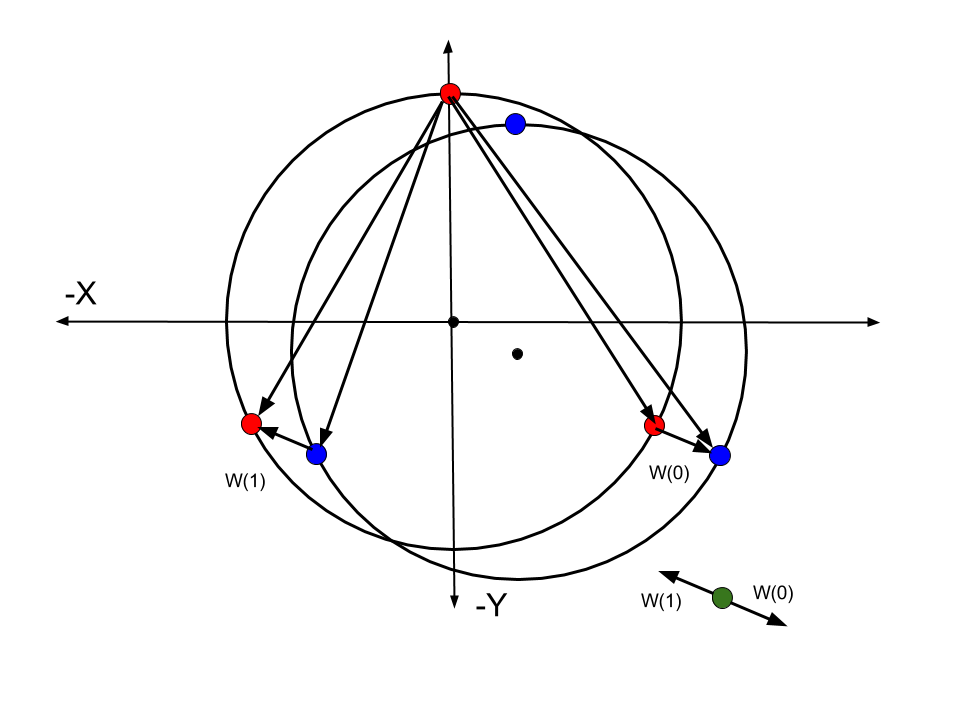
\includegraphics[width=0.45\textwidth]{figures/WobbleDiagram.png}
     \caption{Wobble Vectors from Non-Coincident Axes}
  \label{fig:wobble}
\end{figure}

  Since $\rho < \pi$ by assumption, by $\cref{lemma:ngon}$,
  the set of wobbles $\{\vec{W}(n) | \text{for any n}\}$
  contains at least three vectors,
  at least two of which point in different directions.
  For any point not at the origin, at least one of these vectors moves closer to the
  point and at least one moves further away.

    The set of all lengths in the tetrahelix is a superset of:
    $L = \{|| \vec{R}(n) - \vec{B}(n)||\}$, which, by our choice,
    has at least one longest or shortest
    length.
    $L = \{|| \vec{R}(n) - (\vec{B'}(n) + \vec{W}(n))||\}$ and so
    $L = \{|| (\vec{R}(n) - \vec{B'}(n)) - \vec{W}(n)||\}$.
    But $\vec{R}(n) - \vec{B'}(n)$ is a constant, so the minimax value of $L$ is improved as $||\vec{W}(n)||$
    decreases.  
    By our choice that there is a Blue-to-Red edge that is either a maximum or a minimum,
    this improves the minimax value of the total tetrahelix.
    
    This process can be carried out on both the Blue and Yellow helices
    (perhaps simultaneously) until $\vec{W}(n)$ is
    zero for both, finding a tetrahelix of improved overall minimax value at each step.
    So a tetrahelix is optimal only when $\vec{W}(n) = 0$, and therefore when $D=0$ and
    $\vec{B}(n) = \vec{B'}(n)$, and all three axes are coincident.
\end{proof}

Now that we have shown that axes are conincident and parallel and that the pitches
are the same for all helices, we can assert that any optimum tetrahelix can
be generated with an equation for helices:
\begin{equation}
\label{eq:triple}
\vec{V}_{triple}(n,c) =
\left [
  \begin{tabular}{c}
   $ r_c \cos(n \alpha +  c 2 \pi /3 + \phi_c)$\\
   $ r_c \sin(n \alpha +  c 2 \pi /3 + \phi_c) $\\
   $ \frac{d(n +c / 3)}{3}   $
  \end{tabular}
  \right ],
\end{equation}
\text{where: \qquad}
\begin{tabular}{l}
  $c \in \{0,1,2\}$,
  \end{tabular}      
which would be much more complicated if the axes where not coincident.
Note that we have not yet shown that the relationships of the radius $r_c$ or
the phase $\phi_c$ for the three helices, so we denoted them with a $c$ subscript to show
they are dependent on the color.
We have not yet investigated in the general case the relationships beteween
$\alpha$, $r$, $\phi$ and $d$ in \cref{eq:triple}.
In \cref{sec:parameterizing}, we give a more specific version of this formula which
generates optimal tetrahelices.
We observe that when $\alpha = 0$, the helices are degenerate, having curvature of $0$,
but because of the $\phi_c$ term, they are not collinear.


\begin{figure}
  \centering
     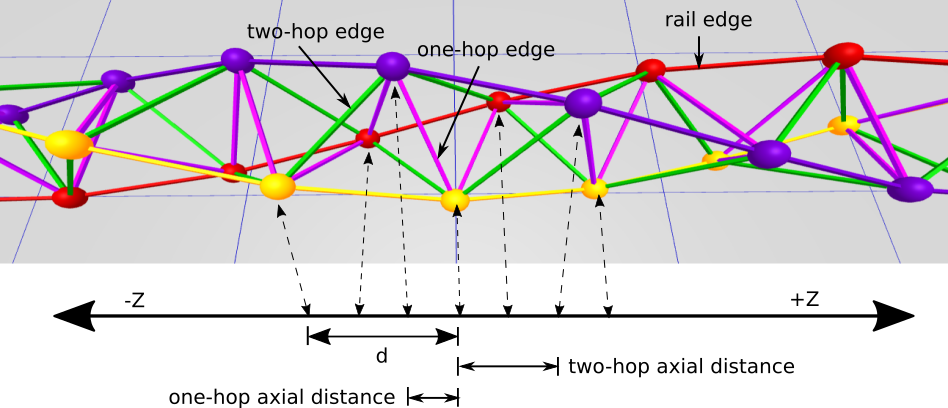
\includegraphics[width=0.45\textwidth]{figures/edge-diagram.png}
     \caption{Edge Naming}
  \label{fig:naming}
\end{figure}

In principle, any three helices generated with \cref{eq:triple}
has at most nine distinct edge length classes. Each edge that connects
two rails potentially has a longer length and shorter length we denote with
a $+$ or $-$. So the classes are $\{ RR, BB, YY, RB_+, RB_-, BY_+, BY_-, RY_+, RY_- \}$.
If when projecting all vertices onto the $z$-axis (dropping the $x$ and $y$ coordinates), the interval
defined by the $z$ axis value of its endpoints contains no other vertices,
we call it a \emph{one-hop} edge, and if it does contain another vertex we
call it a \emph{two-hop} edge, as illustrated in \cref{fig:naming}.
Then there are 
3 rail edges $\{ RR, BB, YY\}$,
3 one-hop lengths $\{ RB_-, BY_-, RY_- \}$ between each pair of 3 rails,
and 3 two-hop
lengths $\{ RB_{+}, BY_+, RY_+ \}$ between each pair of 3 rails,
where the two-hop length is at least the one-hop length.
However, if we symmetrically generate the three helices  with \cref{eq:triple},
many of these lengths will be the same.
In fact, it is possible that there
will be only two distinct such classes. In the purely regular BC helix there is only one length.

\begin{theorem}
  Optimal tetrahelices have the same radius for all three helices.
\end{theorem}
\begin{proof}
To prove this theorem, we exhibit a symmetric tetrahelix (not yet shown to be optimal) which
happens to be a triple helix, that has
the property that all rail edges are equal to all one-hop edges and all two-hop
edges are equal to each other. 
Observe that although we have not get given the formula for the
radii of such a triple helix, there are some values for $r$ and $\alpha$, and $\phi$
in \cref{eq:triple}
for which all the three helices are symmetrically and evenly spaced. Furthermore,
we can choose these values such that the three rail edges are of length $1$ and
so that the one-hop lengths are also all of length $1$, and the two-hop lengths
are slightly longer.

Now consider a tetrahelix in which the radius of one of the helices is different.
By the connections made in a tetrahelix, any increase to a radius increases both
a one-hop and two-hop distance, and any decrease likewise decreases two.
Since there exists a tetrahelix which has only two distinct classes of edge lengths,
the smaller being one-hop = rail, the larger being the two-hop distance, the helix
with a larger radius increases a longest edge without increasing a shortest edges.
Likewise, a helix with a smaller radius decreases a one-hop edge without decreasing
a two-hop edge.  Therefore, a tetrahelix with different radii is not as optimal as some two-class 
tetrahelix generated by \cref{eq:triple}, and so it not optimal. We have not yet
proved that a two-class tetrahelix is optimal, but it suffices to show that there
exists such a better tetrahelix to show that different radii imply a suboptimal
tetrahelix.
\end{proof}

Because an optimal tetrhelix has equivalent radii and equivalent pitch for all three helices,
it has equivalent rail edge lengths. Likewise, there is a single rail angle $\rho$ that
represents the rotation of two vertices connected by a single rail edge, and it is the same
for all three rails.

Now that we have shown that on any optimal tetrahelix the vertices
are on helices of the same axes and pitch, we see that the vertices 
of any optimal tetrahelix will lie on a cylinder, or a circle when the axis dimension
is projected out. Therefore, it is reasonable to now speak of the singular radius $r$
of a tetrahelix as the radius of the cylinder.
We can now go on to
the harder proof about where vertices occur along the $z$-axis.

 We show that, in fact, the vertices must be distributed in even thirds
 along the $z$-axis as they are in the regular BC helix.

 However, we have already shown the rail
 lengths are equal in any optimal tetrahelix.

\begin{figure}
     \centering
     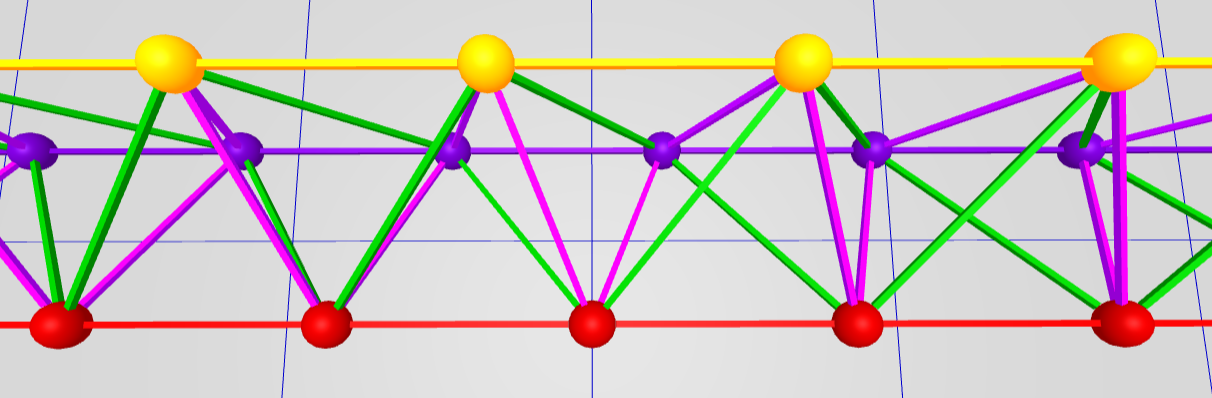
\includegraphics[width=0.45\textwidth]{figures/EquitetrabeamCloseUp.png}
     \caption{Equitetrabeam}
  \label{fig:equitetrabeam}
\end{figure}

\Cref{fig:equitetrabeam} shows the equitetrabeam, which is defined in \cref{sec:equitetrabeam},
but also conveniently illustrates the one-hop and two-hop edge defintions.
The green edges are the two-hop edges and the purple edges are the one-hop edges. Note that the green
edges are slightly longer than the purple edges. In \cref{fig:naming}, which depicts the BC helix,
the two-hop and one-hop edges are of equal length (but the projection onto the $z$-axis, the
axial length, of the two-hop edge is longer than the axial one-hop length.)


\begin{theorem}
  \label{eventhirds}
  An optimal tetrahelix of any rail angle $0 \leq \rho < \pi$ is a triple helix with all vertices evenly spaced at $d/3$ intervals on the $z$ axis.
  Any one tetrahedron in a tetrahelix has $1$ rail edge, $2$ one-hop edges connected to the rail, and $2$ two-hop edges connected to the rail.
  The sixth edge is opposite of the rail edge and is a one-hop edge.
\end{theorem}

\begin{proof}
    Consider a tetrahelix in which the vertices are evenly spaced at
    $d/3$ intervals on the $z$ axis. Every edge is either a rail edge,
    or it makes one hop, or two hops. All of the one-hop
    edges are equal length.  All of the two-hop edges are equal
    length.

    Every vertex is connected to 4 non-rail edges. There is a one-hop edge
    in both the positive and negative $z$ direction. Likewise, there is a two-hop
    edge in both the positive and negative $z$ direction. Let $A$ be the set
    of edge lengths, which has only 3 members, represented by $A = \{o,t,r\}$ for
    the one-hop, two-hop, and rail edge lengths.

    Any attempt to perturb any rail in either $z$ direction lengthens one two-hop edge to $t'$, where $t' > t$
    and shortens one one-hop edge $o' < o$. Let $B = \{o',t' \} \cup A$ be the edge lengths of such a
    perturbed tetrahelix.
    The minimax of $B$ is greater than the minimax of $A$ since there is a single rail length which cannot be both greater
    than $o'$ and $t'$ and less than $o'$ and $t'$.
    Therefore, any optimal tetrahelix has all one-hop edges between all rails equal to each other, and
    all two-hop edges equal to each other, and the $z$ distances between rails equal. Therefore, vertices are
    $d/3$ from each other on the $z$-axis.
\end{proof}

 Note that based on \cref{eventhirds}, there are only 3 possible lengths in an optimal tethrahelix,
 and we are justified in classifying edge lengths as \emph{rail}, \emph{one-hop}, or
\emph{two-hop}. The one-hop edges are the edges between rails that are closest on the $z$-axis, and the two-hop edges are those that skip over a vertex.


Taking all of these results together, 
each helix in an optimal tetrahelix is congruent to the others, shares an axis, is the same radius, and is evenly spaced
axially with the others.
An optimal tetrahelix is therefore a \emph{triple helix}, of a radius we have not yet demonstrated.

\section{Parameterizing Tetrahelices via Rail Angle}
\label{sec:parameterizing}

We seek a formula to generate optimal tetrahelices that accepts a
parameter that allows us to design the tetrahelix conveniently.
Please refer back to \cref{railanglefig}.
The pitch of the helix is an obvious choice, but is not defined when the
curvature is $0$, an important special case. The radius or the axial
distance between two vertices on the same rail are possible choices, but
perhaps the clearest choice is to build formulae that takes as their
input the ``rail angle'' $\rho$. We define $\rho$ to be the angle
formed in the X,Y plane with origin $O$: $\angle \vec{H}(0,0) O \vec{H}(0,1)$ projecting out the
$z$-axis and sighting along the positive $z$a-xis. In other words, $\rho$
controls how far a rail edge of a tetrahelix deviates from being
parallel with the axis, or the ``twistiness'' of the tetrahelix. We use
the parameter $\chi = 1$ to indicate a chirality of counter-clockwise,
and $\chi = -1$ for clockwise. We take our coordinate system to be right-handed.

The quantities $\rho,r,d$ (see \cref{railanglefig}) are related by the expression:

\begin{align*}
  1^2 &= d^2 + (2 r \sin{ \rho / 2})^2 , \text{ or }\\
%%  1 &= d^2 + 4 r^2 (\sin{ \rho / 2})^2 \\
  d^2 &= 1 - 4 r^2 (\sin{ \rho / 2})^2  \text{ .}  \numberthis  \label{railangle} \\
\end{align*}

Checking the important special case of the BC helix, we find that this equation
indeed holds true, treating $d$ in this equation as $3 h_{bc}$ as defined by
Gray and Coxeter, that is, $d_{bc} = 3h_{bc}$, where they are using
$h$ for the axial height from one vertex to
the next of a different color, but we use $d$ to mean distance between vertices of
the  same color.

The rail angle $\rho$ also has the meaning that $2 \pi / \rho$ is the number of
tetraheda in a full revolution of the helix.

In choosing $\rho$, one greatly constrains $r$ and $d$, but does not completely
determine both of them together, so we treat both as additional parameters.

Rewriting our formulation in terms of $\rho$:
\begin{equation}
  \begin{split}
  \label{eq:general}  
\vec{H}_{general}(\chi,n,c,\rho,d_{\rho},r_{\rho}) = \\ 
 \left [
  \begin{tabular}{c}
   $ r_{\rho} \cos(\chi \cdot (n \rho + c(\rho +  2 \pi) /3)) $\\
   $ r_{\rho}  \sin(\chi \cdot (n \rho + c(\rho +  2 \pi) /3)) $\\
   $ d_{\rho} (n + c /3) $
  \end{tabular}
  \right ] \\
   \end{split}
\end{equation}  
\text{where: \qquad} 
\begin{tabular}{l}
  $   1 = d_{\rho}^2 + 4 r_{\rho}^2 (\sin{ \rho / 2})^2 $, and \\
    $\chi \in \{-1,1\}$ \text{.} \\  
\end{tabular}



$\vec{H}_{general}$ forces the user to select three values satisfying \cref{railangle}: $\rho$, $r_{\rho}$, and $d_{\rho}$.

Note that when $\rho = 0$ then $d_{\rho} = 1$, but $r_{\rho}$ is not determined by
\cref{railangle}.

\begin{theorem}
  \label{generalformulaoptimal}
  For rail angles of magnitude at most $\rho_{bc}$, tetrahelices generated by
  $\vec{H}_{general}$ are optimal in terms of minimum maximum (minimax) ratio of member
  length when radius is chosen so that
  the length of the one-hop edge is equal to the rail length.
\end{theorem}


\begin{proof}
By \cref{eventhirds}, we can compute the (at most) three edge-lengths of an optimal
tetrahelix by formulae universally quantified by $n$ and $c$:
\begin{equation}
  \begin{split}
  1 = \text{rail} &= || \vec{H}_{general}(n,c,\rho,d_{\rho},r)  - \\
  &  \vec{H}_{general}(n+1,c,\rho,d_{\rho}),r))  \text{ ,} \\
  \end{split}
\end{equation}
\begin{equation}
  \begin{split}  
  \text{one-hop} &= || \vec{H}_{general}(n,c,\rho,d_{\rho},r)  - \\
  &  \vec{H}_{general}(n,c+1,\rho,d_{\rho},r)) || \text{ and,} \\
  \end{split}  
\end{equation}  
  \begin{equation}
  \begin{split}    
  \text{two-hop} &= || \vec{H}_{general}(n,c,\rho,d_{\rho},r)  - \\
  &  \vec{H}_{general}(n,c+2,\rho,d_{\rho},r)) || \text{ .}\\
  \end{split}  
\end{equation}  

This syntax just represents the Euclidean distance between vertices. Thus:
\begin{equation}
%%  \text{one-hop} &= dist(\vec{H}_{general}(0,0,\rho,d_{\rho}),\vec{H}_{general}(0,1,\rho,d_{\rho},r))  \\  
%%  \text{one-hop}  &= \sqrt{\frac{d_{\rho}^2}{9} + (r\sin(0) - r\sin(\rho/3+1\cdot\frac{2\pi}{3}))^2  +
%%    (r\cos(0) - r\cos(\rho/3 + 1\cdot\frac{2\pi}{3}))^2} \\
%%  \text{one-hop}  &= \sqrt{\frac{d_{\rho}^2}{9} + (0  - r\sin(\rho/3 + \frac{2\pi}{3}))^2  +
%%    (r - r\cos(\rho/3 + \frac{2\pi}{3}))^2} \\
%%  \text{one-hop}  &= \sqrt{\frac{d_{\rho}^2}{9} + r^2\sin^2(\rho/3 + \frac{2\pi}{3})  +
%%    r^2(1 - \cos(\rho/3 + \frac{2\pi}{3}))^2} \\
  %% Formula above checks at sqrt(8/27), 1, 0, and rho_bc, h_bc, r_bc.
  \text{one-hop}  = \sqrt{\frac{d_{\rho}^2}{9} + r^2(\sin^2(\rho/3 + \frac{2\pi}{3})  + (1 - \cos(\rho/3 + \frac{2\pi}{3}))^2)} 
\end{equation}

where: $  d_{\rho}^2 = 1 - 4 r^2 (\sin( \rho / 2)^2$.

%% so we substitute:
%% \begin{align*}
%%   %% Formula above checks at sqrt(8/27), 1, 0, and rho_bc, h_bc, r_bc.  
%%   \text{one-hop}  &= \sqrt{\frac{1}{9}  + r^2(-\frac{4 (\sin^2( \rho / 2))}{9} + \sin^2(\rho/3+ \frac{2\pi}{3})  + (1 - \cos(\rho/3 + \frac{2\pi}{3}))^2)} \text{.}\\
%%   %% Formula above checks at sqrt(8/27), 1, 0, and rho_bc, h_bc, r_bc.    
%% \end{align*}

By similar algebra and trigonometry:
\begin{equation}
  \text{two-hop}  = \sqrt{\frac{4 d_{\rho}^2}{9} +  \sin^2(2\rho/3 + \frac{4\pi}{3})  + (1 - \cos(2\rho/3 + \frac{4\pi}{3}))^2)} \text{.}\\
\end{equation}


By definition of minimax edge length optimality, we are trying to minimize:
\[
\frac{\max{\{1,\text{one-hop}(r),\text{two-hop}(r)}\}}{\min{\{1,\text{one-hop}(r),\text{two-hop}(r)}\}} \text{.}
\]
But since $\text{two-hop}(r) \geq \text{one-hop}(r)$, this is equivalent to:
\[
 \frac{   \max \{1,\text{two-hop}(r)\}}
      {   \min \{1,\text{one-hop}(r)\}} \text{.}
\]
This quantity will be equal to one of:
\begin{equation}
  \frac{\text{two-hop}(r)}{1},
\frac{1}{\text{one-hop}(r)},
\frac{\text{two-hop}(r)}{\text{one-hop}(r)} \text{.}
\label{eq:ratioset}
\end{equation}

We know that both one-hop($r$) and two-hop($r$) increase monotonically and continuously with increasing $r$.
By inspection, it seems likely that we will minimize this set by equating $\text{one-hop}(r)$ or $\text{two-hop}(r)$
to 1, but to be absolutely sure and to decide which one, we must examine the partial derivative of the ratio
 $\frac{\text{two-hop}(r)}{\text{one-hop}(r)}$ in this range.

Although complicated, we can use Mathematica to investigate
the partial derivative of $\frac{\text{two-hop}(r)}{\text{one-hop}(r)}$ with respect
to the radius to be able to understand how to choose the radius to form the minimax optimum.

Let:
\begin{equation}
  f_{\rho} = -\frac{4 (\sin^2( \rho / 2))}{9} \text{,}
  \end{equation}
\begin{equation}
  g_{\rho} = -\frac{16 (\sin^2( \rho / 2))}{9} \text{,}
\end{equation}
\begin{equation}
  j_{\rho} = \sin^2(\rho/3+ \frac{2\pi}{3})  + (1 - \cos(\rho/3 + \frac{2\pi}{3}))^2 \text{,}
\end{equation}
and:
\begin{equation}
  k_{\rho} = \sin^2(2\rho/3 + \frac{4\pi}{3})  + (1 - \cos(2\rho/3 + \frac{4\pi}{3}))^2 \text{.}
\end{equation}

Then:
\begin{equation}
  \begin{split}
  \frac{\text{two-hop}(r)}{ \text{one-hop}(r)}  &=
  \frac{\sqrt{\frac{4}{9}  + r^2(g_{\rho}+ j_{\rho})}}
       {\sqrt{\frac{1}{9} +r^2(f_{\rho}+k_{\rho}) }} \text{.}
  \end{split}       
\end{equation}



By graph inspection using Mathematica (\url{https://github.com/PubInv/tetrahelix/blob/master/tetrahelix.nb}), we see the partial derivative of this with respect to
radius $r$ is always negative, for any $\rho \leq \rho_{bc}$. When the rail angle approaches
$\pi$, corresponding to going almost to the other side of the tetrahelix, this is not necessarily true, hence the
limitation in our statement of the theorem is meaningful.
Since the partial derivative of  $\frac{\text{two-hop}(r)}{\text{one-hop}(r)}$ with respect to the
radius $r$ is negative for all $\rho$ up until $\rho_{bc}$, this ratio goes down
as the radius goes up, and 
we minimize the maximum edge-length ratio by choosing the largest radius
up until one-hop $= 1$, the rail-edge length. If we attempted to further increase the radius
we would not be optimal, because the ratio $\frac{\text{two-hop}(r)}{1}$ would become the
largest ratio in our set of ratios \cref{eq:ratioset}.

Therefore, we decrease the minimax length
of the whole system as we increase the radius
up to the point that the shorter, one-hop distance is equal to the rail-length, $1$.
In order to optimize the whole system so long as $\rho \leq \rho_{bc}$,
we equate one-hop to $1$ to find the optimum radius:


\begin{equation}
  1 =  \sqrt{
    \begin{tabular}{ccc}
    $  \frac{1}{9} $ & + & $ r_{opt}^2(-\frac{4 (\sin^2( \rho / 2))}{9} \; \;+ $\\
$      \sin^2(\rho/3+ \frac{2\pi}{3}) $ & + & $ (1 - \cos(\rho/3 + \frac{2\pi}{3}))^2) $
    \end{tabular}
    }
\end{equation}    
from which it follows that:

\begin{equation}
  r_{opt} = \frac{2}{\sqrt{\frac{9}{2} \cdot ( \sqrt{3} sin(\rho/3) + \cos(\rho/3)) + \cos(\rho)+ 8 }} \text{ .} \numberthis  \label{eqrhoopt}
\end{equation}


We can now give a formula for $ d_{opt} $ computed from $\rho, r_{opt}$ via the rail angle equation \cref{railangle}:

\begin{equation}
  %%  d_{opt}^2 &= 1 - 4 (\frac{2}{\sqrt{\frac{9}{2} \cdot ( \sqrt{3} \sin(\rho/3) + \cos(\rho/3)) + \cos(\rho)+ 8 }})^2 (\sin{ \rho / 2})^2   \\
  d_{opt}^2 = 1 - 4 (r_{opt})^2 (\sin{ \rho / 2})^2,
\end{equation}
which we can expand,
\begin{equation}
%%  d_{opt}^2 &= 1 - 4 \frac{4(\sin{ \rho / 2})^2}{\frac{9}{2} \cdot ( \sqrt{3} \sin(\rho/3) + \cos(\rho/3)) + \cos(\rho)+ 8 }    \\
  d_{opt}^2 = 1 - \frac{16(\sin{ \rho / 2})^2}{9 ( \sqrt{3} \sin(\rho/3) + \cos(\rho/3)) + \cos(\rho)+ 8 }    \\
\end{equation}
and then rewrite:
\begin{equation}
%%  d_{opt}^2 &= 1 - \frac{16 \sin^2(\rho / 2) }{ \cos(\rho) + 9( \sqrt{3} \sin(\rho/3) + \cos(\rho/3)) + 8 }   \\
    d_{opt} = \sqrt{1 - \frac{16 \sin^2(\rho / 2) }{ \cos(\rho) + 9( \sqrt{3} \sin(\rho/3) + \cos(\rho/3)) + 8 }}  \text{ .}  \numberthis  \label{dopt}  \\      
\end{equation}



Thus, by computing $r_{opt}$  and $d_{opt}$ as a function of $\rho$ from this equation, we can construct minimax optimal tetrahelix where $0 \leq \rho \leq \rho_{bc}$.
%% Add here references to these equations.
\end{proof}

\section{The Inradius}

\begin{figure}
     \centering
     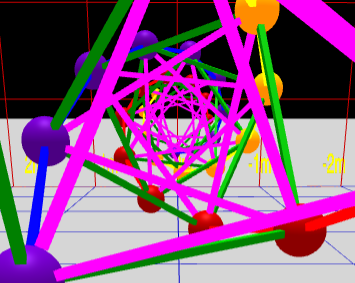
\includegraphics[width=0.45\textwidth]{figures/AxialView.png}
     \caption{Axial view of a BC-Helix}
  \label{axialview}     
\end{figure}

Since the axes are parallel, we may define the \emph{inradius}, represented by the letter $i$, of a
tetrahelix to be the radius of the largest
cylinder parallel to this axis that is surrounded by each tetrahelix and penetrated by no edge.


If we look down the axis of an optimal tetrahelix as shown in \cref{axialview}, it happens that only
the one-hop edges
(rendered in purple in our software)
comes closest to the axis. In other words, they define the radius of the incircle of the
projection, or the radius of a cylinder that would just fit inside the tetrahelix.
A formula for the inradius of the tetrahelix is useful if you are designing it as a structure that bears something internally,
such as a firehose, a pipe, or
a ladder for a human. The inradius $r_{in}(\rho)$ of
an optimal tetrahelix is a remarkably simple function of the radius $r$ and the rail angle $\rho$:
\begin{equation}
  \label{eq:inradius}
  r_{in}(\rho) = r \sin{\frac{\pi - \rho}{6}} \text{ ,}
\end{equation}
which can be seen from the trigonometry of a diagram of the projected one-hop edges
connecting four sequentially numbered vertices, shown in \cref{fig:projectiondiagram}.

\begin{figure}
     \centering
     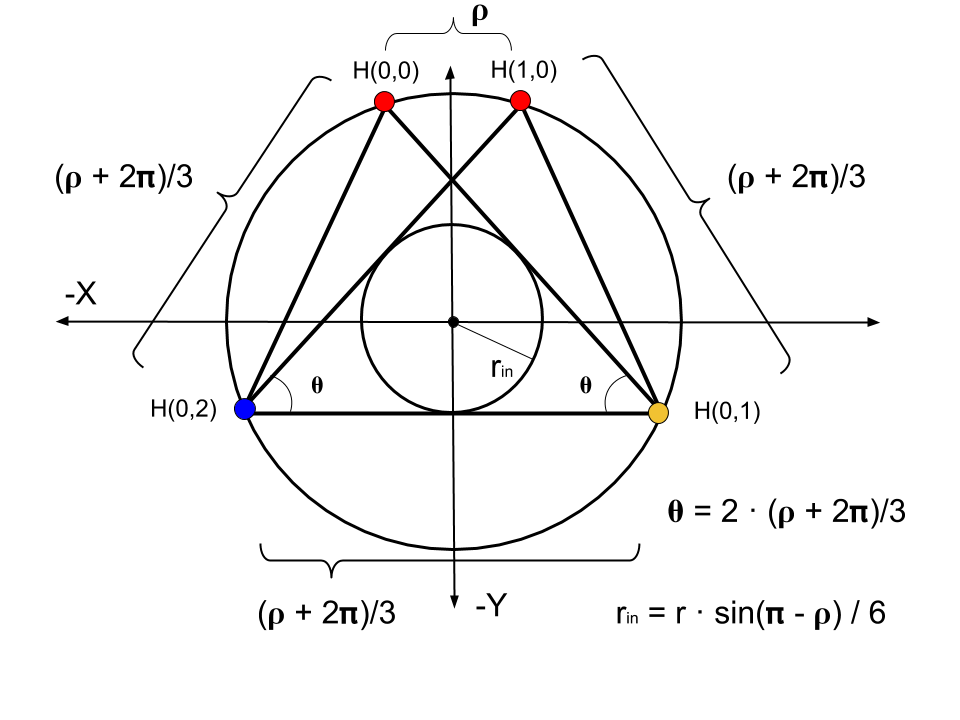
\includegraphics[width=0.45\textwidth]{figures/ProjectionDiagram.png}
     \caption{General One-hop Projection Diagram}
  \label{fig:projectiondiagram}
\end{figure}

From this equation, with the help of symbolic computation, we observe that inradius of the BC helix of unit rail length is $r_{in(\rho_{bc})} = \frac{3}{10\sqrt{2}} \approx 0.21$.

\section{The Equitetrabeam}
\label{sec:equitetrabeam}

Just as $\vec{H}_{general}$ constructs the BC helix (with careful and non-obvious choices of parameters)
which is an important
special case due to its regularity, it constructs an additional special
(degenerate) case when the rail angle $\rho = 0$
and $d = 1$ (the edge-length), where the cross sectional area is
an equilateral triangle of unchanging orientation, as shown in \cref{fig:equitetrabeam} and at the rear of \cref{fig:series}.
We call this the \emph{equitetrabeam}. It is not possible to generate an equitetrabeam from 
\cref{graycoxeter}
without the split into three rails introduced by \cref{eq:colored} and completed in  \cref{eq:general}.



\begin{corollary}
  The equitetrabeam with minimum maximum edge ratio is produced
  \newline by $\vec{H}_{general}$ when $ r = \sqrt{\frac{8}{27}} $ and the longest member is $\frac{2}{\sqrt{3}}$,
  which is less than $16\%$ longer
  than the shortest member.
\end{corollary}

\begin{proof}
Choosing $d = 1$ and $\rho = 0$ we use  \cref{eqrhoopt} to find the radius of 
optimal minimax difference. Substituting into  \cref{eq:general} and setting one-hop\footnote{Before developing the optimal solution  \cref{eqrhoopt} we found another interesting but non-optimal tetrabeam of zero curvature
by setting
the mean of one-hop and two-hop to 1 ($(\text{one-hop} + \text{two-hop})/2 = 1$),
  which gives $r = \sqrt{35}/4$ and
  three length classes of $\frac{11}{12}, \frac{12}{12}, \frac{13}{12}$.}
 to $1$
gives:
%% \begin{align*}
%%   1  &=  \sqrt{\frac{1}{9} + 3r^2} \\
%% \end{align*}  
%% and solving for $r$, gives
%% \begin{align*}
%%    r  &= \sqrt{\frac{8}{27}} \approx 0.54 \text{.}\\
%% \end{align*}
$ 1  =  \sqrt{\frac{1}{9} + 3r^2} $, or $ r  = \sqrt{\frac{8}{27}}$. This radius
produces a two-hop edge length of $\frac{2}{\sqrt{3}} \approx 1.1547$.
\end{proof}


The inradius of the equitetrabeam of unit
rail length from both  \cref{eq:inradius} and the fact that the inradius of
an equilateral triangle is half the circumradius is $\sqrt{\frac{8}{27}}/2$, or $\frac{\sqrt{6}}{9}$.


In \cref{fig:series}, the furthest tetrahelix is the optimal equitetrabeam.
\Cref{fig:equitetrabeam} is a closeup of an equitetrabeam.

To the extent that we value tetrabeams (that is, tetrahelices with a rail angle of $0$,
and therefore zero curvature) as mathematical or engineering objects,
we have motivated the development of $\vec{H}_{general}$ as a transformation of $\vec{V}(n)$ defined by
 \cref{graycoxeter} from Gray and Coxeter. It is difficult to see how
the $\vec{V}(n)$ 
formulation could ever give rise to a continuum producing the tetrabeam,
since setting the angle in that equation to zero can produce only collinear points.

The equitetrabeam may possibly be a novel construction.
The fact that 6 members meet in a single point would have been a manufacturing disadvantage that
may have dissuaded structural engineers from using this geometry.
However, the advent of additive manufacturing, such as 3D printing, and the invention of two
distinct concentric multimember joints\cite{song2003spherical,HamlinSandersonCMS} has improved that situation.

Note that the equitetrabeam has chirality, which becomes important in our attempt to build a
continuum of tetrahelices.

\section{An Untwisted Continuum}
\label{sec:continuum}


We observe that  \cref{eqrhoopt,dopt} compute $r_{opt}$ and $d_{opt}$ which
create an optimal tetrahelix for any rail angle $\rho$ between $0$, which
gives the equitetrabeam and
$\rho_{bc} \approx 35.43 \degree$, which gives the BC helix.

 Because the equitetrabeam which has a rail angle of $0$ still has
 chirality, that is, one still must decide to connect the one-hop edge to
 the clockwise or the counter-clockwise vertex, it is not possible to build
 a smooth continuum where $\rho$ transitions from positive to negative
 which remains optimal. One can use a negative $\rho$ in $\vec{H}_{general}$
 but it does not produce minimax optimal tetrahelices. In other words,
 untwisting a counter-clockwise tetrahelix to rail angle $0$ and then going
even further does produce a clockwise tetrahelix, but one in which the
 one-hop and two-hop lengths in the wrong places, that is, two-hop
 becomes shorter than one-hop.
 Likewise, $\rho > \rho_{bc}$ generates
 a tetrahelix, but we have not proved or investigated optimality in that range.
 
 The pitch of a helix for a known $z$-axis travel $d$
 is trivial (see \cref{pitcheqn}).
If one is varying $\rho$ to obtain a desired pitch
from \cref{dopt} and \cref{pitcheqn} it is not so simple.
However, the pitch increases monotonically and smoothly with decreasing $\rho$, so
\cref{pitcheqn} can be easily solved numerically with a Newton-Raphson
solver, as we do on our website.
For a pitch at least $ p \geq \frac{3  \sqrt{2}  \pi}{\sqrt{5}\rho_{bc}} \approx 9.64 $,
using \cref{dopt} produces minimax optimal tetrahelices.

In this way, a rail angle can be chosen for any desired (sufficiently large) pitch, yielding
the optimum radius, the one-hop length, and the two-hop length that an engineer needs to
construct a physical structure.

The curvature of a rail helix is formally given by:
\begin{equation}
  \frac{|r_{\rho}|}{r_{\rho}^2 + (d_{\rho}/\rho)^2} \text{ .}
\end{equation}
which goes to $0$ as $\rho$ approaches $0$ (the equitetrabeam.)
As $\rho$ increase up to $\rho_{bc}$ the curvature increases smoothly until the BC Helix is reached.

Perhaps surprisingly, the optimal untwisting is accomplished only by
changing the length of the two-hop member, leaving the one-hop member
and rail length equivalent within this continuum.\footnote{Before
deriving  \cref{eqrhoopt}, we created a continuum by
using a linear interpolation between the optimal radius for the
equitetrabeam and the BC Helix. This minimax optimum of this simpler
approach was at most 1\% worse than the optimum computed by
\cref{eqrhoopt}.}
 However, it should
be noted that an engineer or architect may also use $\vec{H}_{general}$ 
directly and interactively via \url{https://pubinv.github.io/tetrahelix/},
and that minimax length optimality is a
mathematical starting point rather than the final word on the beauty and utility of
physical structures. For example, a structural engineer might increase a
radius past optimality in order to resist buckling.
%% Add a figure here of a deep beam and of an arch.

If an equitetrabeam were actually
used as a beam, an engineer might start with the optimal tetrabeam and
dilate it in one dimension to stiffen the beam by deepening it. Similarly, simple
length changes curve the equitetrabeam into an arch.
The ``colored'' approach of  \cref{eq:general} exposes these possibilities
more than the approach of  \cref{graycoxeter}.

Trusses and space frames remain an important design field in
mechanical and structural engineering\cite{mikulas1985sequentially},
including deployable and moving trusses\cite{claypool2012readily}.

\begin{figure}
  \centering
     \includegraphics[width=0.5\textwidth]{figures/MedCantedCropped.png}
     \caption{7-Tet Tetrobot in relaxed, or BC helix configuration}
     \includegraphics[width=0.5\textwidth]{figures/EquitetrabeamCropped.png}
     \caption{The Equitetrabeam: Fully Untwisted 7-Tet Tetrobot in Hexapod Configuration}
     \label{fig:tetrobot}
\end{figure}

\section{Utility for Robotics}

Starting twenty years ago, Sanderson\cite{sanderson1996modular},
Hamlin,\cite{TetrobotBook}, Lee\cite{lee2002dynamic}, and others
 created a style of robotics based on changing
the lengths of members joined at the center of a joint, thereby
creating a connection to pure geometry. More recently, NASA has
experimented with tensegrities\cite{NTRT,chen2017soft}, a different point in the
same design spectrum. In particular, the tetrahelix is related to the
tetraspline\cite{mirletz2014} concept used as a physical concept of a tensegrity robot.
Although tensegrities are not member-for-member isomorphic to the tetrahelix
as the tetrobot is, they often use repeated tetrahedral cells, so this
work of pure geometry has some applied relevance to them.

As suggested by Buckminster Fuller, the most convenient geometries to
consider are those that have regular member lengths, in order to
facilitate the inexpensive manufacture and construction of the robot.
In a plane, the octet truss\cite{richard1961synergetic} is such a geometry, but in a line, the
Boerdijk-Coxeter helix is a regular structure.

However, a robot must move, and so it is interesting to consider the
transmutations of these regular geometries. Developing a functional
gait for our physical Tetrobot was in fact the motivation
for this work.
By changing only the length of the longer members that connect two
distinct rails (the two-hop members), we can dynamically untwist a physical Tetrobot
forming the Boerdijk-Coxeter configuration into the equitetrabeam which rests flat on the plane,
as shown in \cref{fig:tetrobot}.

By untwisting the tetrahelix so that is has a planar surface resting on the ground,
we may consider each vertex touching the ground a foot or pseudopod. A robot can thus
become a hexapod or $n$-pod tetrobot, and the already well-developed approaches to
hexapod gaits may be applied to make the robot walk or crawl.

\section{Conclusion}

There exists a continuum of minimax edge-length optimal tetrahelices
having as one end the Boerdijk-Coxeter Helix and at  the
other end a completely untwisted tetrahelix with equilateral cross
section and planar faces, the equitetrabeam.
By changing the length of only one out of three members by less than $16\%$,
all configurations in the continuum may be reached.
All such optimal may be generated by a simple equation giving coordinates or by
selecting approprate edge-lengths.
All such optimal tetrahelices are proven to be triple helices.
A machine, such as a robot or a variable-geometry truss, that can change
the length of some of its members by $16\%$ can thus twist and untwist itself.
A completely regular Tetrobot can untwist itself to create a planar
face on the ground for locomotion.
With a numeric solution, a designer may choose
a rotation angle to obtain an optimal tetrahelix design
of any pitch, including rational ones.

\section{Contact and Getting Involved}

The Tetrobot Project:\\  
\url{http://pubinv.github.io/tetrobot/} is part of Public Invention,
a free-libre, open-source research, hardware, and software project that welcomes volunteers.
To assist, contact:\\
\href{mailto:read.robert@gmail.com}{read.robert@gmail.com}.

\bibliographystyle{asmems4}
\bibliography{IEEEabrv,gluss}

\end{document}

TODO:

** Add the Mathematica notebook to the github repo (after cleaning up) and reference. -- done
** Redo the proof
** make sure our diagrams are right-handed.

May want to read this article:

http://ieeexplore.ieee.org/abstract/document/7759811/?reload=true


http://epubs.siam.org/toc/sjaabq/1/1

Reread everything, especially the new parts.


Note:

I do not believe it is worth providing a proof of (b or 2b) result of lemma ngon.
However, here are my notes if it becomes important:

Basically by using the distributive nature of mod and the definition of a helix,
the cardinality of the set can remove the PI factor in the sin(x) = sin(x mod 2PI).
Then we know that a, b, and 2 are integers.  We can provide the cardinality is
the residue of [n*a mod 2b], which becomes an integer modulus operation.
if a = k2, you can factor out 2, which has no bearing on cardinality. the
cardinality is the | { nk mod b } | = b.

If a is odd, it is | { n(2k+1) mod 2b) | = 2b.  How do we know we can
  reach each integer < 2b?  By Bezout's Identity there exists x,y, nax + yc = gcd(a,c).
  Take c = 2b.
  But gcd(a,c) = 1, because they are relatively prime. Take but
  So we have ax + y2b = 1.  But (ax + y2b) mod 2b = ax mod 2b. Now  (nax) mod 2b = n,
  up until y = 2b -1.
